% This is the Reed College LaTeX thesis template. Most of the work
% for the document class was done by Sam Noble (SN), as well as this
% template. Later comments etc. by Ben Salzberg (BTS). Additional
% restructuring and APA support by Jess Youngberg (JY).
% Your comments and suggestions are more than welcome; please email
% them to cus@reed.edu
%
% See http://web.reed.edu/cis/help/latex.html for help. There are a
% great bunch of help pages there, with notes on
% getting started, bibtex, etc. Go there and read it if you're not
% already familiar with LaTeX.
%
% Any line that starts with a percent symbol is a comment.
% They won't show up in the document, and are useful for notes
% to yourself and explaining commands.
% Commenting also removes a line from the document;
% very handy for troubleshooting problems. -BTS

% As far as I know, this follows the requirements laid out in
% the 2002-2003 Senior Handbook. Ask a librarian to check the
% document before binding. -SN

%%
%% Preamble
%%
% \documentclass{<something>} must begin each LaTeX document
\documentclass[12pt,twoside]{reedthesis}
% Packages are extensions to the basic LaTeX functions. Whatever you
% want to typeset, there is probably a package out there for it.
% Chemistry (chemtex), screenplays, you name it.
% Check out CTAN to see: http://www.ctan.org/
%%
\usepackage{graphicx,latexsym}
\usepackage[french]{babel} 
\usepackage{amsmath}
\usepackage{amssymb,amsthm}
\usepackage{xcolor}
\usepackage{eso-pic}
\usepackage{longtable,booktabs,setspace}
\usepackage{chemarr} %% Useful for one reaction arrow, useless if you're not a chem major
\usepackage[hyphens]{url}
\usepackage{tikz}
\usetikzlibrary{calc}
\newcommand\HRule{\rule{\textwidth}{1pt}}
% Added by CII
\usepackage{hyperref}
\usepackage{lmodern}
\usepackage{float}
\floatplacement{figure}{H}
% End of CII addition
\usepackage{rotating}

% Next line commented out by CII
%%% \usepackage{natbib}
% Comment out the natbib line above and uncomment the following two lines to use the new
% biblatex-chicago style, for Chicago A. Also make some changes at the end where the
% bibliography is included.
%\usepackage{biblatex-chicago}
%\bibliography{thesis}


% Added by CII (Thanks, Hadley!)
% Use ref for internal links
\renewcommand{\hyperref}[2][???]{\autoref{#1}}
\def\chapterautorefname{Chapter}
\def\sectionautorefname{Section}
\def\subsectionautorefname{Subsection}
% End of CII addition

% Added by CII
\usepackage{caption}
\captionsetup{width=5in}
% End of CII addition

% \usepackage{times} % other fonts are available like times, bookman, charter, palatino


% To pass between YAML and LaTeX the dollar signs are added by CII
\title{THÈSE}
\author{Keurcien LUU}
\labo{Techniques de l'Ingénierie Médicale et de la Complexité - Informatique,
Mathématiques et Applications de Grenoble (TIMC-IMAG)}
% The month and year that you submit your FINAL draft TO THE LIBRARY (May or December)
\date{31 octobre 2017}
\division{Mathematics and Natural Sciences}
\advisor{Michael BLUM}
%If you have two advisors for some reason, you can use the following
% Uncommented out by CII
% End of CII addition

%%% Remember to use the correct department!
\department{Ingénierie de la Santé, de la Cognition et Environnement (EDISCE)}
% if you're writing a thesis in an interdisciplinary major,
% uncomment the line below and change the text as appropriate.
% check the Senior Handbook if unsure.
%\thedivisionof{The Established Interdisciplinary Committee for}
% if you want the approval page to say "Approved for the Committee",
% uncomment the next line
%\approvedforthe{Committee}

% Added by CII
%%% Copied from knitr
%% maxwidth is the original width if it's less than linewidth
%% otherwise use linewidth (to make sure the graphics do not exceed the margin)
\makeatletter
\def\maxwidth{ %
  \ifdim\Gin@nat@width>\linewidth
    \linewidth
  \else
    \Gin@nat@width
  \fi
}
\makeatother

\renewcommand{\contentsname}{Table of Contents}
% End of CII addition

\setlength{\parskip}{0pt}

% Added by CII

\providecommand{\tightlist}{%
  \setlength{\itemsep}{0pt}\setlength{\parskip}{0pt}}

\Acknowledgements{
Je tiens à remercier mes collègues Kevin Caye, Thomas Dias-Alves, Thomas
Karaouzène et Florian Privé, avec qui j'ai partagé ces trois années de
thèse et de qui j'ai beaucoup appris.
}

\Dedication{

}

\Preface{
This is an example of a thesis setup to use the reed thesis document
class (for LaTeX) and the R bookdown package, in general.
}

\Abstract{
The preface pretty much says it all. \par  Second paragraph of abstract
starts here.
}

% End of CII addition
%%
%% End Preamble
%%
%

\usepackage{amsthm}
\newtheorem{theorem}{Theorem}[section]
\newtheorem{lemma}{Lemma}[section]
\theoremstyle{definition}
\newtheorem{definition}{Definition}[section]
\newtheorem{corollary}{Corollary}[section]
\newtheorem{proposition}{Proposition}[section]
\theoremstyle{definition}
\newtheorem{example}{Example}[section]
\theoremstyle{remark}
\newtheorem*{remark}{Remark}
\begin{document}

% Everything below added by CII
      \maketitle
  
  \frontmatter % this stuff will be roman-numbered
  \pagestyle{empty} % this removes page numbers from the frontmatter

      \begin{acknowledgements}
      Je tiens à remercier mes collègues Kevin Caye, Thomas Dias-Alves, Thomas
      Karaouzène et Florian Privé, avec qui j'ai partagé ces trois années de
      thèse et de qui j'ai beaucoup appris.
    \end{acknowledgements}
  
      \begin{preface}
      This is an example of a thesis setup to use the reed thesis document
      class (for LaTeX) and the R bookdown package, in general.
    \end{preface}
  
      \hypersetup{linkcolor=black}
    \setcounter{tocdepth}{2}
    \tableofcontents
  
      \listoftables
  
      \listoffigures
  
      \begin{abstract}
      The preface pretty much says it all. \par  Second paragraph of abstract
      starts here.
    \end{abstract}
  
  
  \mainmatter % here the regular arabic numbering starts
  \pagestyle{fancyplain} % turns page numbering back on

  \chapter*{Introduction}\label{introduction}
  \addcontentsline{toc}{chapter}{Introduction}
  
  \chapter{État de l'art}\label{etat-de-lart}
  
  \begin{itemize}
  \item
    ACP en génétique des populations
  \item
    Partie III: R package pcadapt
  \end{itemize}
  
  \section{Analyse en Composantes Principales
  parcimonieuse}\label{analyse-en-composantes-principales-parcimonieuse}
  
  \section{Bootstrap ACP}\label{bootstrap-acp}
  
  \section{Contexte}\label{contexte}
  
  It's easy to create a list. It can be unordered like
  
  \begin{itemize}
  \tightlist
  \item
    Item 1
  \item
    Item 2
  \end{itemize}
  
  or it can be ordered like
  
  \begin{enumerate}
  \def\labelenumi{\arabic{enumi}.}
  \tightlist
  \item
    Item 1
  \item
    Item 2
  \end{enumerate}
  
  Notice that I intentionally mislabeled Item 2 as number 4.
  \emph{Markdown} automatically figures this out! You can put any numbers
  in the list and it will create the list. Check it out below.
  
  To create a sublist, just indent the values a bit (at least four spaces
  or a tab). (Here's one case where indentation is key!)
  
  \begin{enumerate}
  \def\labelenumi{\arabic{enumi}.}
  \tightlist
  \item
    Item 1
  \item
    Item 2
  \item
    Item 3
  
    \begin{itemize}
    \tightlist
    \item
      Item 3a
    \item
      Item 3b
    \end{itemize}
  \end{enumerate}
  
  \section{Tests multiples}\label{tests-multiples}
  
  \section{Contrôle du taux de fausse
  découverte}\label{controle-du-taux-de-fausse-decouverte}
  
  Le taux de fausse découverte, correspond à la proportion de faux
  positifs parmi les positifs. En notant \(FP\) le nombre de faux
  positifs, \(FP\) le nombre de vrais positifs, on définit le taux de
  fausse découverte \(FDR\) par :
  \[ FDR = \mathbb{E}\Big[\frac{FP}{TP + FP} 1_{FP+TP > 0}\Big] \] -
  Référence cours de Christophe Giraud
  
  q-value, bonferroni, benjamini-hochberg La figure suivante donne les
  comparaisons entre les différentes procédures de correction :
  
  \emph{Now for the correct way:}
  
  Here is the first sentence. Here is another sentence. Here is the last
  sentence to end the paragraph.
  
  This should be a new paragraph.
  
  \section{R chunks}\label{r-chunks}
  
  When you click the \textbf{Knit} button above a document will be
  generated that includes both content as well as the output of any
  embedded \textbf{R} code chunks within the document. You can embed an
  \textbf{R} code chunk like this (\texttt{cars} is a built-in \textbf{R}
  dataset):
  
  \begin{Shaded}
  \begin{Highlighting}[]
  \KeywordTok{summary}\NormalTok{(cars)}
  \end{Highlighting}
  \end{Shaded}
  
  \begin{verbatim}
  ##      speed           dist       
  ##  Min.   : 4.0   Min.   :  2.00  
  ##  1st Qu.:12.0   1st Qu.: 26.00  
  ##  Median :15.0   Median : 36.00  
  ##  Mean   :15.4   Mean   : 42.98  
  ##  3rd Qu.:19.0   3rd Qu.: 56.00  
  ##  Max.   :25.0   Max.   :120.00
  \end{verbatim}
  
  \section{Inline code}\label{inline-code}
  
  If you'd like to put the results of your analysis directly into your
  discussion, add inline code like this:
  
  \begin{quote}
  The \texttt{cos} of \(2 \pi\) is 1.
  \end{quote}
  
  Another example would be the direct calculation of the standard
  deviation:
  
  \begin{quote}
  The standard deviation of \texttt{speed} in \texttt{cars} is 5.2876444.
  \end{quote}
  
  One last neat feature is the use of the \texttt{ifelse} conditional
  statement which can be used to output text depending on the result of an
  \textbf{R} calculation:
  
  \begin{quote}
  The standard deviation is less than 6.
  \end{quote}
  
  Note the use of \texttt{\textgreater{}} here, which signifies a
  quotation environment that will be indented.
  
  As you see with \texttt{\$2\ \textbackslash{}pi\$} above, mathematics
  can be added by surrounding the mathematical text with dollar signs.
  More examples of this are in {[}Mathematics and Science{]} if you
  uncomment the code in \protect\hyperlink{math}{Math}.
  
  \section{Including plots}\label{including-plots}
  
  You can also embed plots. For example, here is a way to use the base
  \textbf{R} graphics package to produce a plot using the built-in
  \texttt{pressure} dataset:
  
  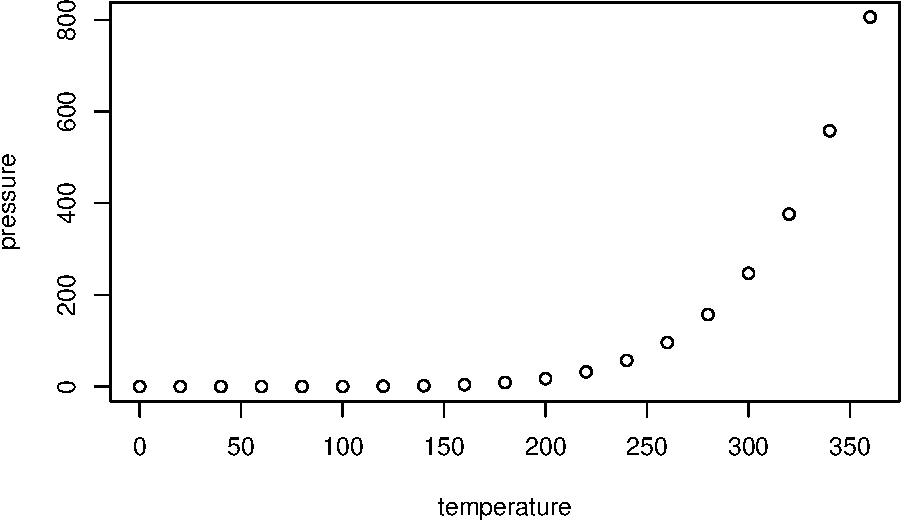
\includegraphics{thesis_files/figure-latex/pressure-1.pdf}
  
  Note that the \texttt{echo=FALSE} parameter was added to the code chunk
  to prevent printing of the \textbf{R} code that generated the plot.
  There are plenty of other ways to add chunk options. More information is
  available at \url{http://yihui.name/knitr/options/}.
  
  Another useful chunk option is the setting of \texttt{cache=TRUE} as you
  see here. If document rendering becomes time consuming due to long
  computations or plots that are expensive to generate you can use knitr
  caching to improve performance. Later in this file, you'll see a way to
  reference plots created in \textbf{R} or external figures.
  
  \hypertarget{loading-and-exploring-data}{\section{Loading and exploring
  data}\label{loading-and-exploring-data}}
  
  Included in this template is a file called \texttt{flights.csv}. This
  file includes a subset of the larger dataset of information about all
  flights that departed from Seattle and Portland in 2014. More
  information about this dataset and its \textbf{R} package is available
  at \url{http://github.com/ismayc/pnwflights14}. This subset includes
  only Portland flights and only rows that were complete with no missing
  values. Merges were also done with the \texttt{airports} and
  \texttt{airlines} data sets in the \texttt{pnwflights14} package to get
  more descriptive airport and airline names.
  
  We can load in this data set using the following command:
  
  \begin{Shaded}
  \begin{Highlighting}[]
  \NormalTok{flights <-}\StringTok{ }\KeywordTok{read.csv}\NormalTok{(}\StringTok{"data/flights.csv"}\NormalTok{)}
  \end{Highlighting}
  \end{Shaded}
  
  The data is now stored in the data frame called \texttt{flights} in
  \textbf{R}. To get a better feel for the variables included in this
  dataset we can use a variety of functions. Here we can see the
  dimensions (rows by columns) and also the names of the columns.
  
  \begin{Shaded}
  \begin{Highlighting}[]
  \KeywordTok{dim}\NormalTok{(flights)}
  \end{Highlighting}
  \end{Shaded}
  
  \begin{verbatim}
  ## [1] 52808    16
  \end{verbatim}
  
  \begin{Shaded}
  \begin{Highlighting}[]
  \KeywordTok{names}\NormalTok{(flights)}
  \end{Highlighting}
  \end{Shaded}
  
  \begin{verbatim}
  ##  [1] "month"        "day"          "dep_time"     "dep_delay"   
  ##  [5] "arr_time"     "arr_delay"    "carrier"      "tailnum"     
  ##  [9] "flight"       "dest"         "air_time"     "distance"    
  ## [13] "hour"         "minute"       "carrier_name" "dest_name"
  \end{verbatim}
  
  Another good idea is to take a look at the dataset in table form. With
  this dataset having more than 50,000 rows, we won't explicitly show the
  results of the command here. I recommend you enter the command into the
  Console \textbf{\emph{after}} you have run the \textbf{R} chunks above
  to load the data into \textbf{R}.
  
  \begin{Shaded}
  \begin{Highlighting}[]
  \KeywordTok{View}\NormalTok{(flights)}
  \end{Highlighting}
  \end{Shaded}
  
  While not required, it is highly recommended you use the \texttt{dplyr}
  package to manipulate and summarize your data set as needed. It uses a
  syntax that is easy to understand using chaining operations. Below I've
  created a few examples of using \texttt{dplyr} to get information about
  the Portland flights in 2014. You will also see the use of the
  \texttt{ggplot2} package, which produces beautiful, high-quality
  academic visuals.
  
  We begin by checking to ensure that needed packages are installed and
  then we load them into our current working environment:
  
  \begin{Shaded}
  \begin{Highlighting}[]
  \CommentTok{# List of packages required for this analysis}
  \NormalTok{pkg <-}\StringTok{ }\KeywordTok{c}\NormalTok{(}\StringTok{"dplyr"}\NormalTok{, }\StringTok{"ggplot2"}\NormalTok{, }\StringTok{"knitr"}\NormalTok{, }\StringTok{"bookdown"}\NormalTok{, }\StringTok{"devtools"}\NormalTok{, }\StringTok{"simulate"}\NormalTok{, }\StringTok{"data.table"}\NormalTok{)}
  \CommentTok{# Check if packages are not installed and assign the}
  \CommentTok{# names of the packages not installed to the variable new.pkg}
  \NormalTok{new.pkg <-}\StringTok{ }\NormalTok{pkg[!(pkg %in%}\StringTok{ }\KeywordTok{installed.packages}\NormalTok{())]}
  \CommentTok{# If there are any packages in the list that aren't installed,}
  \CommentTok{# install them}
  \NormalTok{if (}\KeywordTok{length}\NormalTok{(new.pkg))}
    \KeywordTok{install.packages}\NormalTok{(new.pkg, }\DataTypeTok{repos =} \StringTok{"http://cran.rstudio.com"}\NormalTok{)}
  \CommentTok{# Load packages (thesisdown will load all of the packages as well)}
  \KeywordTok{library}\NormalTok{(thesisdown)}
  \end{Highlighting}
  \end{Shaded}
  
  \clearpage
  
  The example we show here does the following:
  
  \begin{itemize}
  \item
    Selects only the \texttt{carrier\_name} and \texttt{arr\_delay} from
    the \texttt{flights} dataset and then assigns this subset to a new
    variable called \texttt{flights2}.
  \item
    Using \texttt{flights2}, we determine the largest arrival delay for
    each of the carriers.
  \end{itemize}
  
  \begin{Shaded}
  \begin{Highlighting}[]
  \NormalTok{flights2 <-}\StringTok{ }\NormalTok{flights %>%}\StringTok{ }
  \StringTok{  }\KeywordTok{select}\NormalTok{(carrier_name, arr_delay)}
  \NormalTok{max_delays <-}\StringTok{ }\NormalTok{flights2 %>%}\StringTok{ }
  \StringTok{  }\KeywordTok{group_by}\NormalTok{(carrier_name) %>%}
  \StringTok{  }\KeywordTok{summarize}\NormalTok{(}\DataTypeTok{max_arr_delay =} \KeywordTok{max}\NormalTok{(arr_delay, }\DataTypeTok{na.rm =} \OtherTok{TRUE}\NormalTok{))}
  \end{Highlighting}
  \end{Shaded}
  
  A useful function in the \texttt{knitr} package for making nice tables
  in \emph{R Markdown} is called \texttt{kable}. It is much easier to use
  than manually entering values into a table by copying and pasting values
  into Excel or LaTeX. This again goes to show how nice reproducible
  documents can be! (Note the use of \texttt{results="asis"}, which will
  produce the table instead of the code to create the table.) The
  \texttt{caption.short} argument is used to include a shorter title to
  appear in the List of Tables.
  
  \begin{Shaded}
  \begin{Highlighting}[]
  \KeywordTok{kable}\NormalTok{(max_delays, }
        \DataTypeTok{col.names =} \KeywordTok{c}\NormalTok{(}\StringTok{"Airline"}\NormalTok{, }\StringTok{"Max Arrival Delay"}\NormalTok{),}
        \DataTypeTok{caption =} \StringTok{"Maximum Delays by Airline"}\NormalTok{,}
        \DataTypeTok{caption.short =} \StringTok{"Max Delays by Airline"}\NormalTok{,}
        \DataTypeTok{longtable =} \OtherTok{TRUE}\NormalTok{,}
        \DataTypeTok{booktabs =} \OtherTok{TRUE}\NormalTok{)}
  \end{Highlighting}
  \end{Shaded}
  
  \begin{longtable}[t]{lr}
  \caption[Max Delays by Airline]{\label{tab:maxdelays}Maximum Delays by Airline}\\
  \toprule
  Airline & Max Arrival Delay\\
  \midrule
  Alaska Airlines Inc. & 338\\
  American Airlines Inc. & 1539\\
  Delta Air Lines Inc. & 651\\
  Frontier Airlines Inc. & 575\\
  Hawaiian Airlines Inc. & 407\\
  \addlinespace
  JetBlue Airways & 273\\
  SkyWest Airlines Inc. & 421\\
  Southwest Airlines Co. & 694\\
  United Air Lines Inc. & 472\\
  US Airways Inc. & 347\\
  Virgin America & 366\\
  \bottomrule
  \end{longtable}
  
  The last two options make the table a little easier-to-read.
  
  We can further look into the properties of the largest value here for
  American Airlines Inc. To do so, we can isolate the row corresponding to
  the arrival delay of 1539 minutes for American in our original
  \texttt{flights} dataset.
  
  \begin{Shaded}
  \begin{Highlighting}[]
  \NormalTok{flights %>%}\StringTok{ }\KeywordTok{filter}\NormalTok{(arr_delay ==}\StringTok{ }\DecValTok{1539}\NormalTok{, }
                    \NormalTok{carrier_name ==}\StringTok{ "American Airlines Inc."}\NormalTok{) %>%}
  \StringTok{  }\KeywordTok{select}\NormalTok{(-}\KeywordTok{c}\NormalTok{(month, day, carrier, dest_name, hour, }
              \NormalTok{minute, carrier_name, arr_delay))}
  \end{Highlighting}
  \end{Shaded}
  
  \begin{verbatim}
  ##   dep_time dep_delay arr_time tailnum flight dest air_time distance
  ## 1     1403      1553     1934  N595AA   1568  DFW      182     1616
  \end{verbatim}
  
  We see that the flight occurred on March 3rd and departed a little after
  2 PM on its way to Dallas/Fort Worth. Lastly, we show how we can
  visualize the arrival delay of all departing flights from Portland on
  March 3rd against time of departure.
  
  \begin{Shaded}
  \begin{Highlighting}[]
  \NormalTok{flights %>%}\StringTok{ }\KeywordTok{filter}\NormalTok{(month ==}\StringTok{ }\DecValTok{3}\NormalTok{, day ==}\StringTok{ }\DecValTok{3}\NormalTok{) %>%}
  \StringTok{  }\KeywordTok{ggplot}\NormalTok{(}\KeywordTok{aes}\NormalTok{(}\DataTypeTok{x =} \NormalTok{dep_time, }\DataTypeTok{y =} \NormalTok{arr_delay)) +}\StringTok{ }\KeywordTok{geom_point}\NormalTok{()}
  \end{Highlighting}
  \end{Shaded}
  
  \begin{figure}[htbp]
  \centering
  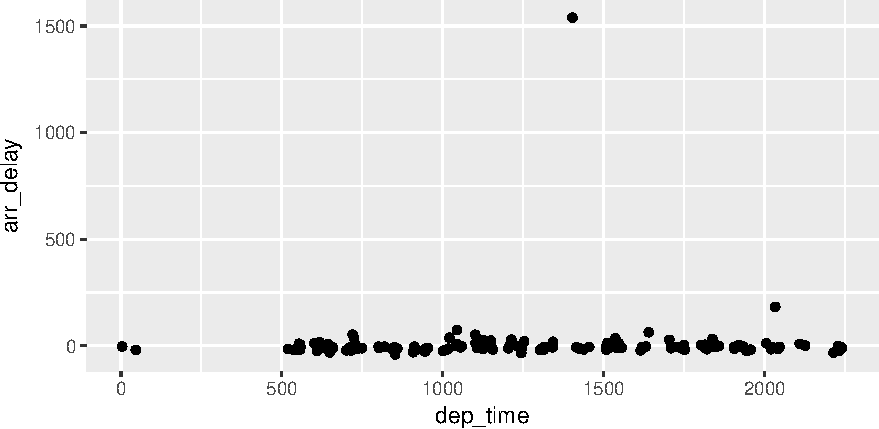
\includegraphics{thesis_files/figure-latex/march3plot-1.pdf}
  \caption{\label{fig:march3plot}\(\beta\)}
  \end{figure}
  
  \section{Additional resources}\label{additional-resources}
  
  \begin{itemize}
  \item
    \emph{Markdown} Cheatsheet -
    \url{https://github.com/adam-p/markdown-here/wiki/Markdown-Cheatsheet}
  \item
    \emph{R Markdown} Reference Guide -
    \url{https://www.rstudio.com/wp-content/uploads/2015/03/rmarkdown-reference.pdf}
  \item
    Introduction to \texttt{dplyr} -
    \url{https://cran.rstudio.com/web/packages/dplyr/vignettes/introduction.html}
  \item
    \texttt{ggplot2} Documentation -
    \url{http://docs.ggplot2.org/current/}
  \end{itemize}
  
  \chapter{Adaptation locale}\label{adaptation-locale}
  
  Une population est dite localement adaptée à son environnement si elle a
  connu une évolution différente de celles qu'ont connu les autres
  populations de la même espèce, et ce, en réponse des pressions
  sélectives
  
  \hypertarget{math}{\section{Math}\label{math}}
  
  \TeX~is the best way to typeset mathematics. Donald Knuth designed
  \TeX~when he got frustrated at how long it was taking the typesetters to
  finish his book, which contained a lot of mathematics. One nice feature
  of \emph{R Markdown} is its ability to read LaTeX code directly.
  
  If you are doing a thesis that will involve lots of math, you will want
  to read the following section which has been commented out. If you're
  not going to use math, skip over or delete this next commented section.
  
  \section{Chemistry 101: Symbols}\label{chemistry-101-symbols}
  
  Chemical formulas will look best if they are not italicized. Get around
  math mode's automatic italicizing in LaTeX by using the argument
  \texttt{\$\textbackslash{}mathrm\{formula\ here\}\$}, with your formula
  inside the curly brackets. (Notice the use of the backticks here which
  enclose text that acts as code.)
  
  So, \(\mathrm{Fe_2^{2+}Cr_2O_4}\) is written
  \texttt{\$\textbackslash{}mathrm\{Fe\_2\^{}\{2+\}Cr\_2O\_4\}\$}.
  
  \noindent Exponent or Superscript: \(\mathrm{O^-}\)
  
  \noindent Subscript: \(\mathrm{CH_4}\)
  
  To stack numbers or letters as in \(\mathrm{Fe_2^{2+}}\), the subscript
  is defined first, and then the superscript is defined.
  
  \noindent Bullet: CuCl \(\bullet\) \(\mathrm{7H_{2}O}\)
  
  \noindent Delta: \(\Delta\)
  
  \noindent Reaction Arrows: \(\longrightarrow\) or
  \(\xrightarrow{solution}\)
  
  \noindent Resonance Arrows: \(\leftrightarrow\)
  
  \noindent Reversible Reaction Arrows: \(\rightleftharpoons\)
  
  \subsection{Typesetting reactions}\label{typesetting-reactions}
  
  You may wish to put your reaction in an equation environment, which
  means that LaTeX will place the reaction where it fits and will number
  the equations for you.
  
  \begin{equation}
    \mathrm{C_6H_{12}O_6  + 6O_2} \longrightarrow \mathrm{6CO_2 + 6H_2O}
    \label{eq:reaction}
  \end{equation}
  
  We can reference this combustion of glucose reaction via Equation
  \eqref{eq:reaction}.
  
  \subsection{Other examples of
  reactions}\label{other-examples-of-reactions}
  
  \(\mathrm{NH_4Cl_{(s)}}\) \(\rightleftharpoons\)
  \(\mathrm{NH_{3(g)}+HCl_{(g)}}\)
  
  \noindent \(\mathrm{MeCH_2Br + Mg}\) \(\xrightarrow[below]{above}\)
  \(\mathrm{MeCH_2\bullet Mg \bullet Br}\)
  
  \section{Physics}\label{physics}
  
  Many of the symbols you will need can be found on the math page
  \url{http://web.reed.edu/cis/help/latex/math.html} and the Comprehensive
  LaTeX Symbol Guide
  (\url{http://mirror.utexas.edu/ctan/info/symbols/comprehensive/symbols-letter.pdf}).
  
  \section{Biology}\label{biology}
  
  You will probably find the resources at
  \url{http://www.lecb.ncifcrf.gov/~toms/latex.html} helpful, particularly
  the links to bsts for various journals. You may also be interested in
  TeXShade for nucleotide typesetting
  (\url{http://homepages.uni-tuebingen.de/beitz/txe.html}). Be sure to
  read the proceeding chapter on graphics and tables.
  
  \chapter{Introgression adaptative}\label{introgression-adaptative}
  
  \section{Coefficients de métissage globaux et
  locaux}\label{coefficients-de-metissage-globaux-et-locaux}
  
  Étant données des populations ancestrales, il est possible d'estimer
  pour un individu donné, la proportion de son génôme provenant de chacune
  des populations ancestrales. Ces proportions sont connues plus
  communément sous le nom de \emph{coefficients de métissage globaux}. De
  nombreux logiciels existent pour l'estimation de ces coefficients :
  STRUCTURE, ADMIXTURE (Alexander, 2009), LEA (Frichot, 2015), tess3r
  (Caye, 2016). En complément à cette information globale, il peut être
  intéressant de déterminer sur des portions plus petites du génôme, de la
  même manière que dans le cas global, les proportions venant de telle ou
  telle population ancestrale pour chacune de ces portions. Nous parlons
  dans ce cas de \emph{coefficients de métissage locaux}. Encore une fois,
  plusieurs logiciels ont été proposés dans le but d'estimer ces
  coefficients : Hapmix (Price, 2009), EILA (Yang, 2013), LAMP (Thornton,
  2014), loter ou encore RFmix (Maples, 2013).
  
  \section{Introgression}\label{introgression}
  
  L'introgression peut être détectée de différentes façons. Une première
  approche consiste à utiliser les \emph{coefficients de métissage
  locaux}. Les méthodes mentionnées plus haut estiment ces coefficients
  pour chaque individu, permettant de calculer à partir de ceux-ci des
  coefficients de métissage locaux pour chaque population.
  
  \section{Lien entre Analyse en Composantes Principales et métissage
  global.}\label{lien-entre-analyse-en-composantes-principales-et-metissage-global.}
  
  L'un des premiers articles à établir un lien entre l'ACP et les
  coefficients de métissage global fut sur l'interprétation généalogique
  de l'ACP de Gil McVean (McVean, 2009):
  
  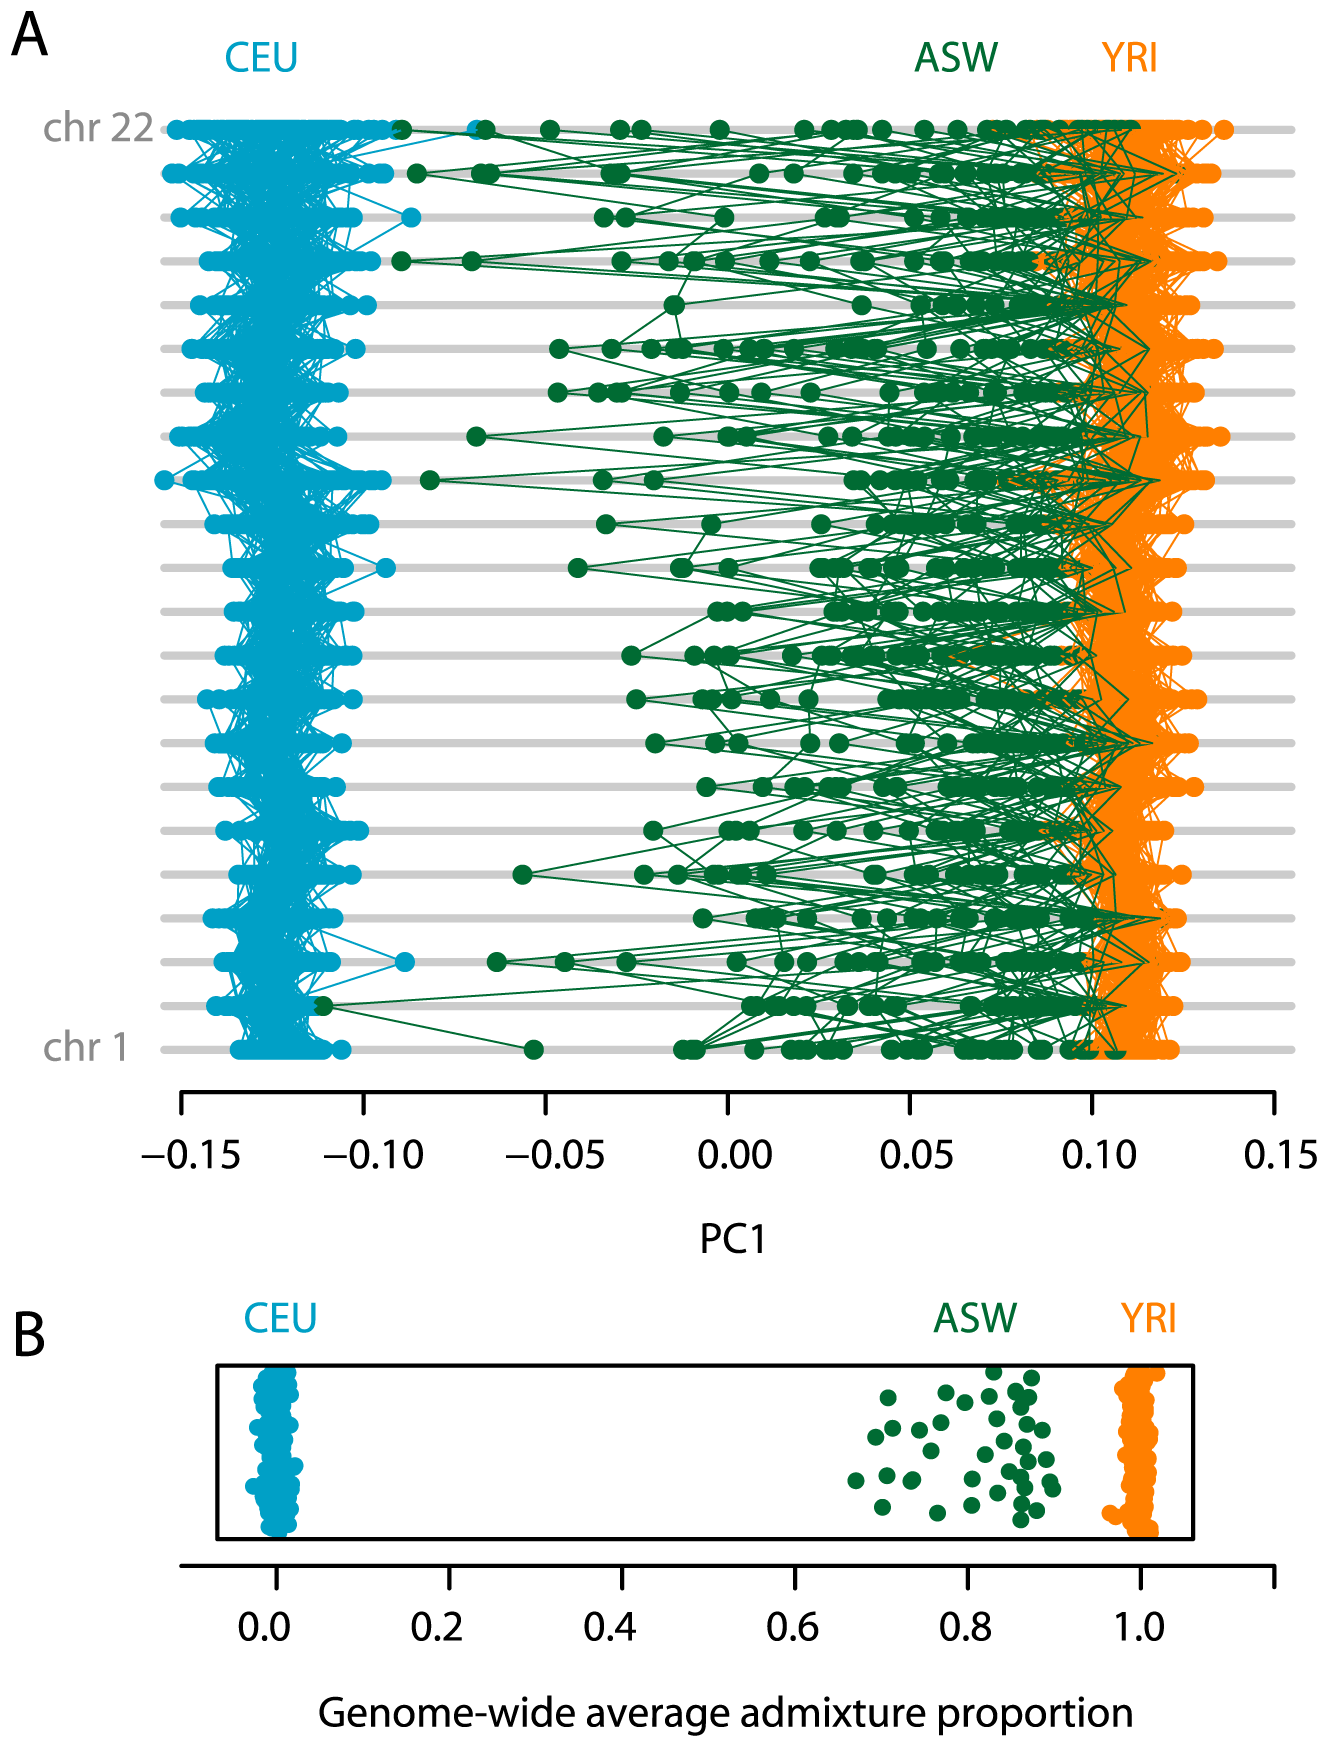
\includegraphics[width=250pt]{figure/mcvean.png}
  
  Pour chacun des 22 chromosomes,
  
  \section{Analyse en Composantes Principales
  locale}\label{analyse-en-composantes-principales-locale}
  
  Notant \(p\) le nombre de marqueurs génétiques, \(i\) un entier compris
  entre \(1\) et \(p\), et \(x_i\) la position génétique (en Morgans) ou
  la position physique (en paires de bases) du \(i\)-ème marqueur
  génétique. Nous définissons pour cet entier \(i\) la fenêtre \(W_i^T\)
  de taille \(T\) et centrée en \(i\) :
  
  \[W_i^T = \{ j \in [|1, p|], |x_i - x_j| \leq T/2 \}\]
  
  \section{Sensibilité à l'imputation des données
  manquantes}\label{sensibilite-a-limputation-des-donnees-manquantes}
  
  \section{Simulations}\label{simulations}
  
  \subsection{Données de peupliers}\label{donnees-de-peupliers}
  
  Le premier jeu de données est issu d'une étude d'introgression
  adaptative chez les peupliers d'Amérique du Nord (Suarez-Gonzalez,
  2016). La simulation d'haplotypes d'individus admixés est effectuée à
  partir des deux populations ancestrales qui y sont présentes. La
  première, \emph{Populus Balsamifera}, est une espèce de peupliers qui
  peuple le nord du continent nord-américain, d'Est en Ouest, et se trouve
  exposée à des conditions climatiques peu clémentes. La seconde,
  \emph{Populus Trichocarpa}, est principalement localisée en Californie,
  et bénéficie d'un climat continental.
  
  Chacune des simulations est constituée de \(50\) haplotypes de la souche
  continentale, de \(50\) haplotyêpes de la souche boréale, ainsi que de
  \(50\) haplotypes d'individus hybrides générés à partir des haplotypes
  ancestraux. Ces haplotypes ancestraux ont été estimés à l'aide du
  logiciel Beagle. 'A partir des positions en paires de base, une carte de
  recombinaison génétique est générée en utilisant le taux de
  recombinaison moyen chez le peuplier. Le taux de recombinaison, noté
  \(\tau_r\), correspond au nombre moyen de paires de bases à parcourir
  pour qu'ait lieu un épisode de recombinaison génétique, \emph{i.e.},
  notant \(L\) la longueur du chromosome en Morgans (\(M\)), et \(N_{bp}\)
  le nombre de paires de bases le constituant, le taux de recombinaison
  génétique pour ce chromosome est donné par la relation:
  
  \[\tau_r = \frac{L}{N_{bp}}\]
  
  Dans ce scénario, les simulations ont été produites en utilisant un taux
  de recombinaison génétique moyen \(\tau_r\) de \(0.05\) centiMorgans par
  million de paire de bases, correspondant à la valeur utilisée par les
  auteurs de l'étude avec le logiciel RASPberry
  (\textit{Recombination via Ancestry Switch Probability}).
  
  \begin{Shaded}
  \begin{Highlighting}[]
  \NormalTok{path <-}\StringTok{ "~/Documents/thesis/git/simulations/introgression/"}
  \NormalTok{output.name <-}\StringTok{ "populus"}
  \NormalTok{recombinationRate <-}\StringTok{ }\FloatTok{0.05} \CommentTok{# in Morgans per Megabase}
  \NormalTok{nSNP <-}\StringTok{ }\DecValTok{50000}
  \NormalTok{ancstrl}\FloatTok{.1} \NormalTok{<-}\StringTok{ }\DecValTok{1}
  \NormalTok{ancstrl}\FloatTok{.2} \NormalTok{<-}\StringTok{ }\DecValTok{3}
  \NormalTok{hyb <-}\StringTok{ }\DecValTok{4}
  \NormalTok{intro.size <-}\StringTok{ }\DecValTok{500}
  \NormalTok{global.ancestry <-}\StringTok{ }\FloatTok{0.1}
  \NormalTok{inverted.ancestry <-}\StringTok{ }\FloatTok{0.5}
  
  \NormalTok{info.map <-}\StringTok{ }\KeywordTok{as.matrix}\NormalTok{(data.table::}\KeywordTok{fread}\NormalTok{(}\KeywordTok{paste0}\NormalTok{(path, output.name, }\StringTok{".map"}\NormalTok{), }
                                          \DataTypeTok{data.table =} \OtherTok{FALSE}\NormalTok{))}
  \NormalTok{H1 <-}\StringTok{ }\KeywordTok{as.matrix}\NormalTok{(data.table::}\KeywordTok{fread}\NormalTok{(}\KeywordTok{paste0}\NormalTok{(path, output.name, }\StringTok{"_H1"}\NormalTok{), }
                                    \DataTypeTok{data.table =} \OtherTok{FALSE}\NormalTok{))}
  \NormalTok{H2 <-}\StringTok{ }\KeywordTok{as.matrix}\NormalTok{(data.table::}\KeywordTok{fread}\NormalTok{(}\KeywordTok{paste0}\NormalTok{(path, output.name, }\StringTok{"_H2"}\NormalTok{), }
                                    \DataTypeTok{data.table =} \OtherTok{FALSE}\NormalTok{))}
  \NormalTok{n.hyb <-}\StringTok{ }\KeywordTok{ncol}\NormalTok{(H1) /}\StringTok{ }\DecValTok{2} 
  
  \NormalTok{### Introgression region}
  \NormalTok{idx <-}\StringTok{ }\KeywordTok{sample}\NormalTok{(}\DecValTok{1}\NormalTok{:nSNP, }\DataTypeTok{size =} \DecValTok{1}\NormalTok{)}
  \NormalTok{beg.reg <-}\StringTok{ }\KeywordTok{max}\NormalTok{(}\DecValTok{1}\NormalTok{, idx -}\StringTok{ }\NormalTok{intro.size)}
  \NormalTok{end.reg <-}\StringTok{ }\KeywordTok{min}\NormalTok{(nSNP, idx +}\StringTok{ }\NormalTok{intro.size)}
  \NormalTok{intro.reg <-}\StringTok{ }\NormalTok{beg.reg:end.reg}
  \end{Highlighting}
  \end{Shaded}
  
  \newpage
  
  \begin{figure}
  
  {\centering 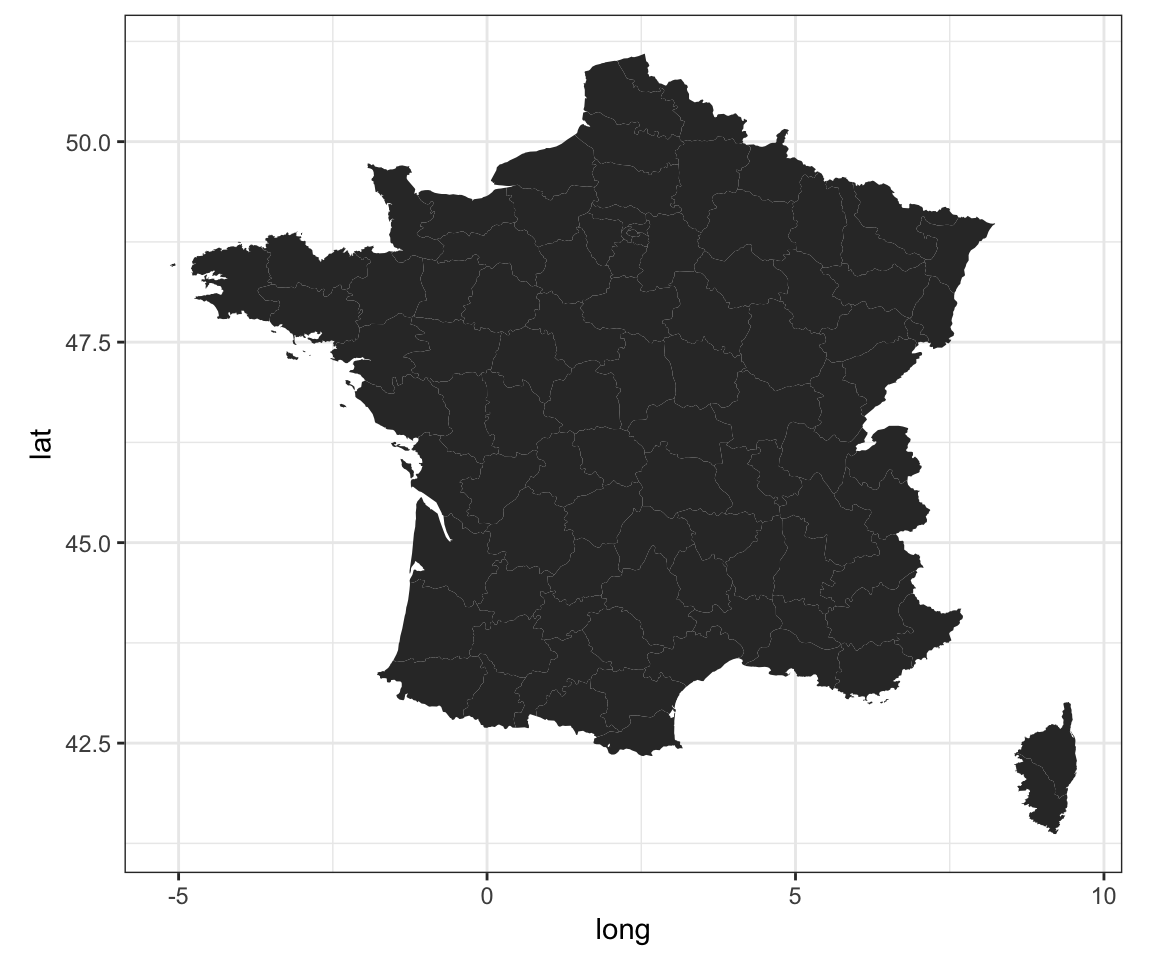
\includegraphics{thesis_files/figure-latex/unnamed-chunk-1-1} 
  
  }
  
  \caption{$\lambda = 0.1$}\label{fig:unnamed-chunk-1}
  \end{figure}
  
  \begin{figure}
  
  {\centering 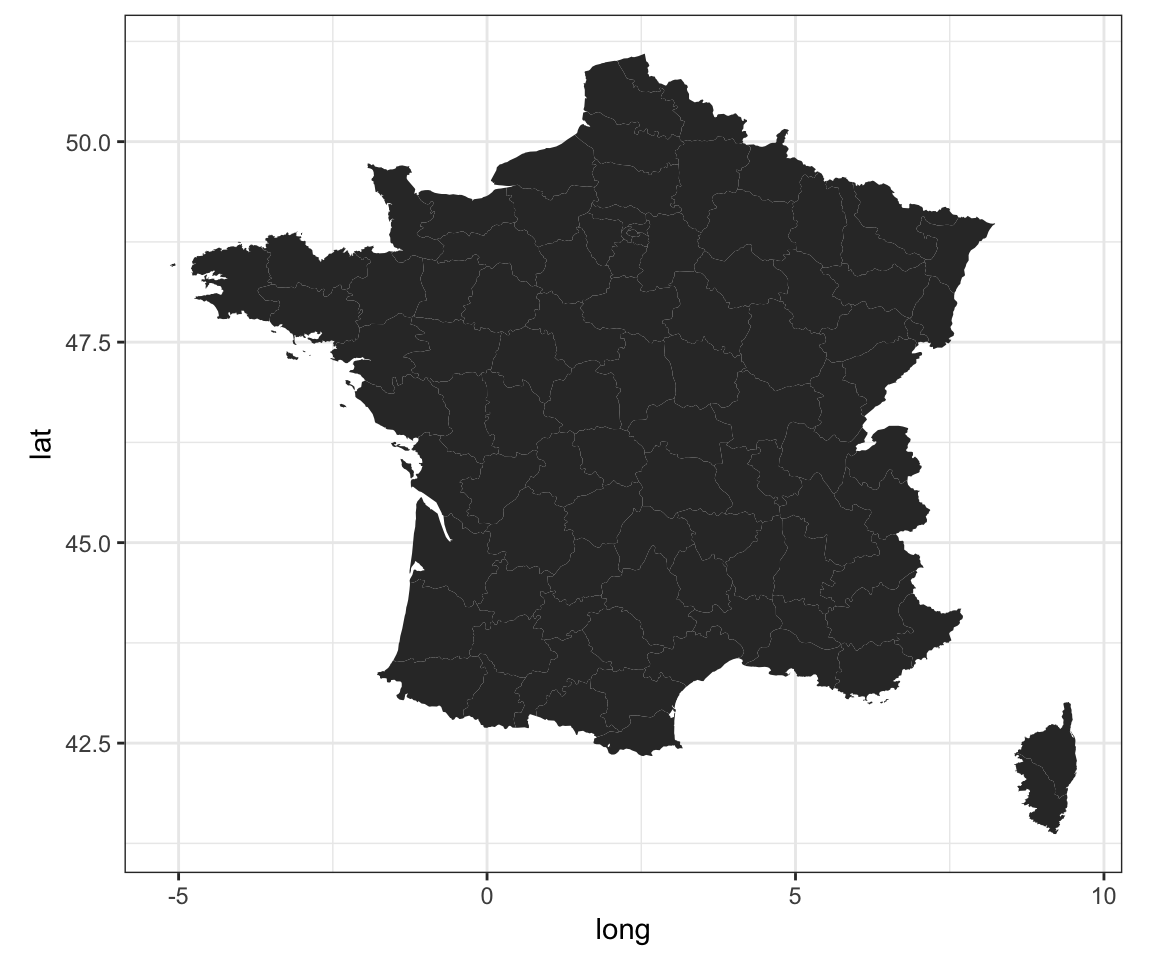
\includegraphics{thesis_files/figure-latex/unnamed-chunk-2-1} 
  
  }
  
  \caption{$\lambda = 10$}\label{fig:unnamed-chunk-2}
  \end{figure}
  
  \begin{figure}
  
  {\centering 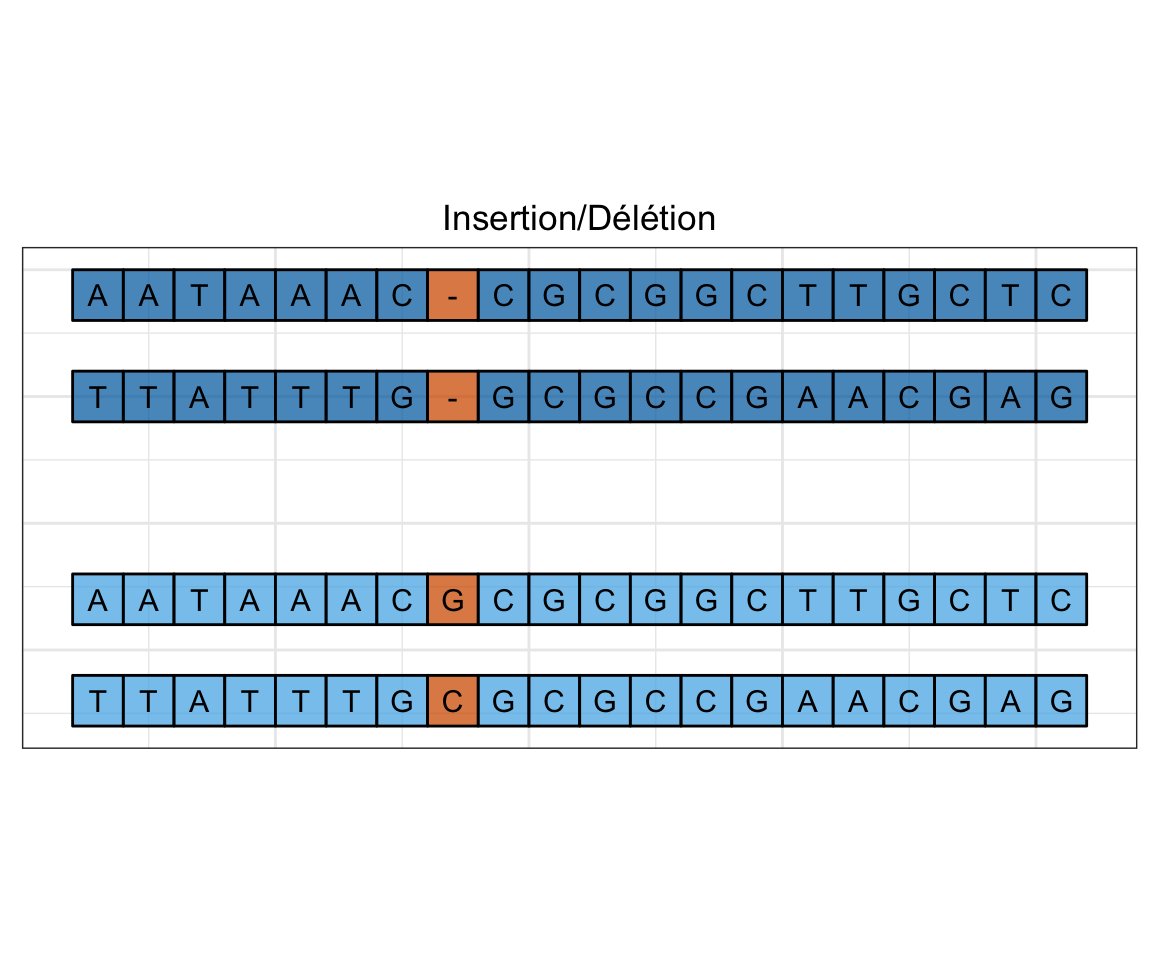
\includegraphics{thesis_files/figure-latex/unnamed-chunk-3-1} 
  
  }
  
  \caption{$\lambda = 50$}\label{fig:unnamed-chunk-3}
  \end{figure}
  
  \newpage
  
  \subsection{Résultats de la comparaison des
  logiciels}\label{resultats-de-la-comparaison-des-logiciels}
  
  \begin{Shaded}
  \begin{Highlighting}[]
  \KeywordTok{setwd}\NormalTok{(}\StringTok{"~/Documents/thesis/git/simulations/introgression/"}\NormalTok{)}
  \NormalTok{output.name <-}\StringTok{ "populus"}
  \NormalTok{recombinationRate <-}\StringTok{ }\FloatTok{0.05} \CommentTok{# in Morgans per Megabase}
  \NormalTok{nSNP <-}\StringTok{ }\DecValTok{50000}
  \NormalTok{ancstrl}\FloatTok{.1} \NormalTok{<-}\StringTok{ }\DecValTok{1}
  \NormalTok{ancstrl}\FloatTok{.2} \NormalTok{<-}\StringTok{ }\DecValTok{3}
  \NormalTok{hyb <-}\StringTok{ }\DecValTok{4}
  \NormalTok{intro.size <-}\StringTok{ }\DecValTok{500}
  \NormalTok{global.ancestry <-}\StringTok{ }\FloatTok{0.1}
  \NormalTok{inverted.ancestry <-}\StringTok{ }\FloatTok{0.5}
  \NormalTok{N <-}\StringTok{ }\DecValTok{10}
  \NormalTok{pop <-}\StringTok{ }\KeywordTok{c}\NormalTok{(}\KeywordTok{rep}\NormalTok{(ancstrl}\FloatTok{.1}\NormalTok{, }\KeywordTok{ncol}\NormalTok{(H1) /}\StringTok{ }\DecValTok{2}\NormalTok{), }
           \KeywordTok{rep}\NormalTok{(ancstrl}\FloatTok{.2}\NormalTok{, }\KeywordTok{ncol}\NormalTok{(H2) /}\StringTok{ }\DecValTok{2}\NormalTok{), }
           \KeywordTok{rep}\NormalTok{(}\DecValTok{4}\NormalTok{, n.hyb))}
  \NormalTok{results <-}\StringTok{ }\KeywordTok{data.frame}\NormalTok{(}\DataTypeTok{Software =} \KeywordTok{c}\NormalTok{(}\StringTok{"pcadapt"}\NormalTok{, }\StringTok{"eila"}\NormalTok{, }\StringTok{"RFMix"}\NormalTok{), }\DataTypeTok{Power =} \KeywordTok{c}\NormalTok{(}\DecValTok{0}\NormalTok{, }\DecValTok{0}\NormalTok{, }\DecValTok{0}\NormalTok{), }\DataTypeTok{FDR =} \KeywordTok{c}\NormalTok{(}\DecValTok{0}\NormalTok{, }\DecValTok{0}\NormalTok{, }\DecValTok{0}\NormalTok{))}
  \NormalTok{info.map <-}\StringTok{ }\KeywordTok{as.matrix}\NormalTok{(data.table::}\KeywordTok{fread}\NormalTok{(}\KeywordTok{paste0}\NormalTok{(path, output.name, }\StringTok{".map"}\NormalTok{), }
                                          \DataTypeTok{data.table =} \OtherTok{FALSE}\NormalTok{))}
  
  \NormalTok{compute.fdr =}\StringTok{ }\NormalTok{function(list, ground.truth)\{}
    \NormalTok{if (}\KeywordTok{length}\NormalTok{(list) ==}\StringTok{ }\DecValTok{0}\NormalTok{)\{}
      \NormalTok{x <-}\StringTok{ }\DecValTok{0}
    \NormalTok{\} else \{}
      \NormalTok{x <-}\StringTok{ }\KeywordTok{sum}\NormalTok{(!(list %in%}\StringTok{ }\NormalTok{ground.truth)) /}\StringTok{ }\KeywordTok{length}\NormalTok{(list)}
    \NormalTok{\}}
    \KeywordTok{return}\NormalTok{(x)}
  \NormalTok{\}}
  
  \NormalTok{compute.power =}\StringTok{ }\NormalTok{function(list, ground.truth)\{}
    \NormalTok{if (}\KeywordTok{length}\NormalTok{(ground.truth) ==}\StringTok{ }\DecValTok{0}\NormalTok{)\{}
      \KeywordTok{warning}\NormalTok{(}\StringTok{"The list of true positives is empty."}\NormalTok{)}
    \NormalTok{\} else \{}
      \NormalTok{x <-}\StringTok{ }\KeywordTok{sum}\NormalTok{(list %in%}\StringTok{ }\NormalTok{ground.truth) /}\StringTok{ }\KeywordTok{length}\NormalTok{(ground.truth)}
    \NormalTok{\}}
    \KeywordTok{return}\NormalTok{(x)}
  \NormalTok{\}}
  
  \NormalTok{for (n.simu in }\DecValTok{21}\NormalTok{:}\DecValTok{30}\NormalTok{)\{}
    \NormalTok{dir.name <-}\StringTok{ }\KeywordTok{paste0}\NormalTok{(}\StringTok{"RFMix_v1.5.4/simu"}\NormalTok{, n.simu, }\StringTok{"/"}\NormalTok{)}
    
    \NormalTok{input.pcadapt <-}\StringTok{ }\KeywordTok{as.matrix}\NormalTok{(data.table::}\KeywordTok{fread}\NormalTok{(}\KeywordTok{paste0}\NormalTok{(dir.name, }\StringTok{"simu.pcadapt"}\NormalTok{), }\DataTypeTok{data.table =} \OtherTok{FALSE}\NormalTok{))}
    \NormalTok{input.eila <-}\StringTok{ }\NormalTok{simulate::}\KeywordTok{eila_from_pcadapt}\NormalTok{(input.pcadapt, pop, }\DataTypeTok{anc1 =} \NormalTok{ancstrl}\FloatTok{.1}\NormalTok{, }\DataTypeTok{anc2 =} \NormalTok{ancstrl}\FloatTok{.2}\NormalTok{, }\DataTypeTok{admixed =} \NormalTok{hyb, }\DataTypeTok{position =} \NormalTok{info.map[, }\DecValTok{2}\NormalTok{])}
    \NormalTok{param <-}\StringTok{ }\KeywordTok{read.table}\NormalTok{(}\KeywordTok{paste0}\NormalTok{(dir.name, }\StringTok{"/parameters.txt"}\NormalTok{))}
    \NormalTok{gt <-}\StringTok{ }\NormalTok{(param$begin):(param$end)}
    
    \NormalTok{### run pcadapt}
    \NormalTok{wsize <-}\StringTok{ }\DecValTok{1000}
    \NormalTok{mmaf <-}\StringTok{ }\FloatTok{0.01}
    \NormalTok{nomap <-}\StringTok{ }\DecValTok{1}\NormalTok{:nSNP}
    \NormalTok{maf <-}\StringTok{ }\NormalTok{pcadapt::}\KeywordTok{cmpt_minor_af}\NormalTok{(input.pcadapt, }\DecValTok{2}\NormalTok{)}
    \NormalTok{proxy.map <-}\StringTok{ }\NormalTok{info.map[}\DecValTok{1}\NormalTok{:nSNP]}
    \NormalTok{filtered.map <-}\StringTok{ }\NormalTok{nomap[maf >=}\StringTok{ }\NormalTok{mmaf]}
    \NormalTok{stat.pcadapt <-}\StringTok{ }\NormalTok{pcadapt::}\KeywordTok{scan.intro}\NormalTok{(input.pcadapt, }\DataTypeTok{K =} \DecValTok{1}\NormalTok{, }\DataTypeTok{pop =} \NormalTok{pop, }
                               \DataTypeTok{ancstrl.1 =} \NormalTok{ancstrl}\FloatTok{.2}\NormalTok{, }
                               \DataTypeTok{ancstrl.2 =} \NormalTok{ancstrl}\FloatTok{.1}\NormalTok{,}
                               \DataTypeTok{admxd =} \NormalTok{hyb,}
                               \DataTypeTok{min.maf =} \NormalTok{mmaf,}
                               \DataTypeTok{window.size =} \NormalTok{wsize,}
                               \DataTypeTok{ploidy =} \DecValTok{2}\NormalTok{,}
                               \DataTypeTok{side =} \StringTok{"middle"}\NormalTok{,}
                               \DataTypeTok{map =} \NormalTok{nomap)}
    
    \NormalTok{### run eila }
    \NormalTok{obj.eila <-}\StringTok{ }\NormalTok{EILA::}\KeywordTok{eila}\NormalTok{(}\DataTypeTok{admixed =} \NormalTok{input.eila$admixed, }\DataTypeTok{anc1 =} \NormalTok{input.eila$anc1,}
                           \DataTypeTok{anc2 =} \NormalTok{input.eila$anc2, }\DataTypeTok{position =} \NormalTok{info.map[, }\DecValTok{1}\NormalTok{], }\DataTypeTok{lambda =} \FloatTok{0.1}\NormalTok{)}
    \NormalTok{loc.anc.eila <-}\StringTok{ }\NormalTok{simulate::}\KeywordTok{haplo_to_ancestry}\NormalTok{(obj.eila$local.ancestry, }\DecValTok{1}\NormalTok{)}
    
    \NormalTok{### run rfmix}
    \NormalTok{allele <-}\StringTok{ }\KeywordTok{paste0}\NormalTok{(}\StringTok{"./simu"}\NormalTok{, n.simu, }\StringTok{"/rfmix_alleles.txt"}\NormalTok{)}
    \NormalTok{classes <-}\StringTok{ }\KeywordTok{paste0}\NormalTok{(}\StringTok{"./simu"}\NormalTok{, n.simu, }\StringTok{"/rfmix_classes.txt"}\NormalTok{)}
    \NormalTok{markerLocation <-}\StringTok{  }\KeywordTok{paste0}\NormalTok{(}\StringTok{"./simu"}\NormalTok{, n.simu, }\StringTok{"/rfmix_markerLocation.txt"}\NormalTok{)}
    \NormalTok{output <-}\StringTok{ }\KeywordTok{paste0}\NormalTok{(}\StringTok{"simu"}\NormalTok{, n.simu, }\StringTok{"/output_simu"}\NormalTok{, n.simu)}
    \NormalTok{window.rfmix <-}\StringTok{ }\FloatTok{0.00002}
    \NormalTok{command <-}\StringTok{ }\KeywordTok{paste}\NormalTok{(}\StringTok{"python2.7 RunRFMix.py PopPhased"}\NormalTok{, allele,  classes,  markerLocation, }\StringTok{"-w"}\NormalTok{, window.rfmix, }\StringTok{"-o"}\NormalTok{, output)}
    \KeywordTok{setwd}\NormalTok{(}\StringTok{"~/Documents/thesis/git/simulations/introgression/RFMix_v1.5.4/"}\NormalTok{)}
    \KeywordTok{system}\NormalTok{(}\DataTypeTok{command =} \NormalTok{command)}
    \KeywordTok{setwd}\NormalTok{(}\StringTok{"~/Documents/thesis/git/simulations/introgression/"}\NormalTok{)}
    \NormalTok{aux.rfmix <-}\StringTok{ }\NormalTok{simulate::}\KeywordTok{rfmix.local.ancestry}\NormalTok{(}\KeywordTok{paste0}\NormalTok{(}\StringTok{"RFMix_v1.5.4/simu"}\NormalTok{, n.simu, }\StringTok{"/output_simu"}\NormalTok{, n.simu, }\StringTok{".0.Viterbi.txt"}\NormalTok{))}
    \NormalTok{loc.anc.rfmix <-}\StringTok{ }\NormalTok{simulate::}\KeywordTok{haplo_to_ancestry}\NormalTok{(aux.rfmix, }\DecValTok{1}\NormalTok{)}
    
    \NormalTok{### FDR}
    \NormalTok{interp <-}\StringTok{ }\KeywordTok{approx}\NormalTok{(filtered.map, stat.pcadapt[[}\DecValTok{1}\NormalTok{]], }\DecValTok{1}\NormalTok{:nSNP)}
    \NormalTok{sd.pcadapt <-}\StringTok{ }\KeywordTok{sd}\NormalTok{(interp$y, }\DataTypeTok{na.rm =} \OtherTok{TRUE}\NormalTok{)}
    \NormalTok{list.pcadapt <-}\StringTok{ }\KeywordTok{which}\NormalTok{(interp$y >}\StringTok{ }\DecValTok{3}\NormalTok{)}
    \NormalTok{results[}\DecValTok{1}\NormalTok{, }\DecValTok{3}\NormalTok{] <-}\StringTok{ }\NormalTok{results[}\DecValTok{1}\NormalTok{, }\DecValTok{3}\NormalTok{] +}\StringTok{ }\KeywordTok{compute.fdr}\NormalTok{(list.pcadapt, gt) /}\StringTok{ }\NormalTok{N}
    \NormalTok{results[}\DecValTok{1}\NormalTok{, }\DecValTok{2}\NormalTok{] <-}\StringTok{ }\NormalTok{results[}\DecValTok{1}\NormalTok{, }\DecValTok{2}\NormalTok{] +}\StringTok{ }\KeywordTok{compute.power}\NormalTok{(list.pcadapt, gt) /}\StringTok{ }\NormalTok{N}
    
    \NormalTok{sd.eila <-}\StringTok{ }\KeywordTok{sd}\NormalTok{(loc.anc.eila, }\DataTypeTok{na.rm =} \OtherTok{TRUE}\NormalTok{)}
    \NormalTok{stat.eila <-}\StringTok{ }\NormalTok{(loc.anc.eila -}\StringTok{ }\KeywordTok{mean}\NormalTok{(loc.anc.eila)) /}\StringTok{ }\NormalTok{sd.eila}
    \NormalTok{list.eila <-}\StringTok{ }\KeywordTok{which}\NormalTok{(stat.eila >}\StringTok{ }\DecValTok{3}\NormalTok{)}
    \NormalTok{results[}\DecValTok{2}\NormalTok{, }\DecValTok{3}\NormalTok{] <-}\StringTok{ }\NormalTok{results[}\DecValTok{2}\NormalTok{, }\DecValTok{3}\NormalTok{] +}\StringTok{ }\KeywordTok{compute.fdr}\NormalTok{(list.eila, gt) /}\StringTok{ }\NormalTok{N}
    \NormalTok{results[}\DecValTok{2}\NormalTok{, }\DecValTok{2}\NormalTok{] <-}\StringTok{ }\NormalTok{results[}\DecValTok{2}\NormalTok{, }\DecValTok{2}\NormalTok{] +}\StringTok{ }\KeywordTok{compute.power}\NormalTok{(list.eila, gt) /}\StringTok{ }\NormalTok{N}
    
    \NormalTok{sd.rfmix <-}\StringTok{ }\KeywordTok{sd}\NormalTok{(loc.anc.rfmix, }\DataTypeTok{na.rm =} \OtherTok{TRUE}\NormalTok{)}
    \NormalTok{stat.rfmix <-}\StringTok{ }\NormalTok{(loc.anc.rfmix -}\StringTok{ }\KeywordTok{mean}\NormalTok{(loc.anc.rfmix)) /}\StringTok{ }\NormalTok{sd.rfmix}
    \NormalTok{list.rfmix <-}\StringTok{ }\KeywordTok{which}\NormalTok{(stat.rfmix >}\StringTok{ }\DecValTok{3}\NormalTok{)}
    \NormalTok{results[}\DecValTok{3}\NormalTok{, }\DecValTok{3}\NormalTok{] <-}\StringTok{ }\NormalTok{results[}\DecValTok{3}\NormalTok{, }\DecValTok{3}\NormalTok{] +}\StringTok{ }\KeywordTok{compute.fdr}\NormalTok{(list.rfmix, gt) /}\StringTok{ }\NormalTok{N}
    \NormalTok{results[}\DecValTok{3}\NormalTok{, }\DecValTok{2}\NormalTok{] <-}\StringTok{ }\NormalTok{results[}\DecValTok{3}\NormalTok{, }\DecValTok{2}\NormalTok{] +}\StringTok{ }\KeywordTok{compute.power}\NormalTok{(list.rfmix, gt) /}\StringTok{ }\NormalTok{N}
  \NormalTok{\}}
  
  
  \NormalTok{ggres <-}\StringTok{ }\KeywordTok{data.frame}\NormalTok{(}\DataTypeTok{Software =} \KeywordTok{rep}\NormalTok{(}\KeywordTok{c}\NormalTok{(}\StringTok{"pcadapt"}\NormalTok{, }\StringTok{"eila"}\NormalTok{, }\StringTok{"RFMix"}\NormalTok{), }\DecValTok{2}\NormalTok{), }\DataTypeTok{Stat =} \KeywordTok{rep}\NormalTok{(}\DecValTok{0}\NormalTok{, }\DecValTok{6}\NormalTok{), }\DataTypeTok{Type =} \KeywordTok{c}\NormalTok{(}\KeywordTok{rep}\NormalTok{(}\StringTok{"Power"}\NormalTok{, }\DecValTok{3}\NormalTok{), }\KeywordTok{rep}\NormalTok{(}\StringTok{"FDR"}\NormalTok{, }\DecValTok{3}\NormalTok{)), }
                      \DataTypeTok{Percent =} \KeywordTok{rep}\NormalTok{(}\DecValTok{0}\NormalTok{, }\DecValTok{6}\NormalTok{))}
  \NormalTok{ggres$Stat[}\DecValTok{1}\NormalTok{:}\DecValTok{3}\NormalTok{] <-}\StringTok{ }\NormalTok{results$Power *}\StringTok{ }\DecValTok{100}
  \NormalTok{ggres$Stat[}\DecValTok{4}\NormalTok{:}\DecValTok{6}\NormalTok{] <-}\StringTok{ }\NormalTok{results$FDR *}\StringTok{ }\DecValTok{100}
  \NormalTok{ggres$Percent <-}\StringTok{ }\KeywordTok{as.numeric}\NormalTok{(}\KeywordTok{format}\NormalTok{(ggres$Stat, }\DataTypeTok{digits =} \DecValTok{2}\NormalTok{))}
  \NormalTok{p0 <-}\StringTok{ }\KeywordTok{ggplot}\NormalTok{(ggres, }\KeywordTok{aes}\NormalTok{(}\DataTypeTok{x =} \NormalTok{Software, }\DataTypeTok{y =} \NormalTok{Stat, }\DataTypeTok{fill =} \KeywordTok{as.factor}\NormalTok{(Type)))}
  \NormalTok{p0 <-}\StringTok{ }\NormalTok{p0 +}\StringTok{ }\KeywordTok{ggtitle}\NormalTok{(}\KeywordTok{expression}\NormalTok{(lambda ==}\StringTok{ }\DecValTok{1}\NormalTok{)) +}\StringTok{ }\KeywordTok{ylab}\NormalTok{(}\StringTok{""}\NormalTok{)}
  \NormalTok{p0 <-}\StringTok{ }\NormalTok{p0 +}\StringTok{ }\KeywordTok{geom_bar}\NormalTok{(}\DataTypeTok{stat =} \StringTok{"identity"}\NormalTok{, }\DataTypeTok{position =} \KeywordTok{position_dodge}\NormalTok{(}\DataTypeTok{width =} \FloatTok{0.9}\NormalTok{))}
  \NormalTok{p0 <-}\StringTok{ }\NormalTok{p0 +}\StringTok{ }\KeywordTok{guides}\NormalTok{(}\DataTypeTok{fill =} \KeywordTok{guide_legend}\NormalTok{(}\DataTypeTok{title =} \StringTok{""}\NormalTok{))}
  \NormalTok{p0 <-}\StringTok{ }\NormalTok{p0 +}\StringTok{ }\KeywordTok{geom_text}\NormalTok{(}\KeywordTok{aes}\NormalTok{(}\DataTypeTok{label =} \NormalTok{Percent), }\DataTypeTok{position =} \KeywordTok{position_dodge}\NormalTok{(}\DataTypeTok{width =} \FloatTok{0.9}\NormalTok{), }
                       \DataTypeTok{color =} \StringTok{"white"}\NormalTok{, }\DataTypeTok{vjust =} \FloatTok{1.4}\NormalTok{, }\DataTypeTok{size =} \DecValTok{5}\NormalTok{)}
  \NormalTok{p0 <-}\StringTok{ }\NormalTok{p0 +}\StringTok{ }\KeywordTok{theme_bw}\NormalTok{() +}\StringTok{ }\KeywordTok{theme}\NormalTok{(}\DataTypeTok{axis.text =} \KeywordTok{element_text}\NormalTok{(}\DataTypeTok{size =} \DecValTok{15}\NormalTok{),}
                                \DataTypeTok{axis.title =} \KeywordTok{element_text}\NormalTok{(}\DataTypeTok{size =} \DecValTok{15}\NormalTok{, }\DataTypeTok{face =} \StringTok{"bold"}\NormalTok{),}
                                \DataTypeTok{title =} \KeywordTok{element_text}\NormalTok{(}\DataTypeTok{size =} \DecValTok{15}\NormalTok{, }\DataTypeTok{face =} \StringTok{"bold"}\NormalTok{),}
                                \DataTypeTok{legend.text =} \KeywordTok{element_text}\NormalTok{(}\DataTypeTok{size =} \DecValTok{15}\NormalTok{),}
                                \DataTypeTok{legend.key.height =} \KeywordTok{unit}\NormalTok{(}\DecValTok{1}\NormalTok{, }\StringTok{"line"}\NormalTok{),}
                                \DataTypeTok{legend.key.width =} \KeywordTok{unit}\NormalTok{(}\DecValTok{3}\NormalTok{, }\StringTok{"line"}\NormalTok{)}
  \NormalTok{)}
  \KeywordTok{print}\NormalTok{(p0)}
  \end{Highlighting}
  \end{Shaded}
  
  \begin{longtable}[]{@{}lcl@{}}
  \caption{\label{tab:inher} Correlation of Inheritance Factors for Parents
  and Child}\tabularnewline
  \toprule
  \begin{minipage}[b]{0.29\columnwidth}\raggedright\strut
  Factors\strut
  \end{minipage} & \begin{minipage}[b]{0.47\columnwidth}\centering\strut
  Correlation between Parents \& Child\strut
  \end{minipage} & \begin{minipage}[b]{0.16\columnwidth}\raggedright\strut
  Inherited\strut
  \end{minipage}\tabularnewline
  \midrule
  \endfirsthead
  \toprule
  \begin{minipage}[b]{0.29\columnwidth}\raggedright\strut
  Factors\strut
  \end{minipage} & \begin{minipage}[b]{0.47\columnwidth}\centering\strut
  Correlation between Parents \& Child\strut
  \end{minipage} & \begin{minipage}[b]{0.16\columnwidth}\raggedright\strut
  Inherited\strut
  \end{minipage}\tabularnewline
  \midrule
  \endhead
  \begin{minipage}[t]{0.29\columnwidth}\raggedright\strut
  Education\strut
  \end{minipage} & \begin{minipage}[t]{0.47\columnwidth}\centering\strut
  -0.49\strut
  \end{minipage} & \begin{minipage}[t]{0.16\columnwidth}\raggedright\strut
  Yes\strut
  \end{minipage}\tabularnewline
  \begin{minipage}[t]{0.29\columnwidth}\raggedright\strut
  Socio-Economic Status\strut
  \end{minipage} & \begin{minipage}[t]{0.47\columnwidth}\centering\strut
  0.28\strut
  \end{minipage} & \begin{minipage}[t]{0.16\columnwidth}\raggedright\strut
  Slight\strut
  \end{minipage}\tabularnewline
  \begin{minipage}[t]{0.29\columnwidth}\raggedright\strut
  Income\strut
  \end{minipage} & \begin{minipage}[t]{0.47\columnwidth}\centering\strut
  0.08\strut
  \end{minipage} & \begin{minipage}[t]{0.16\columnwidth}\raggedright\strut
  No\strut
  \end{minipage}\tabularnewline
  \begin{minipage}[t]{0.29\columnwidth}\raggedright\strut
  Family Size\strut
  \end{minipage} & \begin{minipage}[t]{0.47\columnwidth}\centering\strut
  0.18\strut
  \end{minipage} & \begin{minipage}[t]{0.16\columnwidth}\raggedright\strut
  Slight\strut
  \end{minipage}\tabularnewline
  \begin{minipage}[t]{0.29\columnwidth}\raggedright\strut
  Occupational Prestige\strut
  \end{minipage} & \begin{minipage}[t]{0.47\columnwidth}\centering\strut
  0.21\strut
  \end{minipage} & \begin{minipage}[t]{0.16\columnwidth}\raggedright\strut
  Slight\strut
  \end{minipage}\tabularnewline
  \bottomrule
  \end{longtable}
  
  We can also create a link to the table by doing the following: Table
  \ref{tab:inher}. If you go back to
  \protect\hyperlink{loading-and-exploring-data}{Loading and exploring
  data} and look at the \texttt{kable} table, we can create a reference to
  this max delays table too: Table \ref{tab:maxdelays}. The addition of
  the \texttt{(\textbackslash{}\#tab:inher)} option to the end of the
  table caption allows us to then make a reference to Table
  \texttt{\textbackslash{}@ref(tab:label)}. Note that this reference could
  appear anywhere throughout the document after the table has appeared.
  
  \clearpage
  
  \section{Figures}\label{figures}
  
  If your thesis has a lot of figures, \emph{R Markdown} might behave
  better for you than that other word processor. One perk is that it will
  automatically number the figures accordingly in each chapter. You'll
  also be able to create a label for each figure, add a caption, and then
  reference the figure in a way similar to what we saw with tables
  earlier. If you label your figures, you can move the figures around and
  \emph{R Markdown} will automatically adjust the numbering for you. No
  need for you to remember! So that you don't have to get too far into
  LaTeX to do this, a couple \textbf{R} functions have been created for
  you to assist. You'll see their use below.
  
  In the \textbf{R} chunk below, we will load in a picture stored as
  \texttt{reed.jpg} in our main directory. We then give it the caption of
  ``Reed logo'', the label of ``reedlogo'', and specify that this is a
  figure. Make note of the different \textbf{R} chunk options that are
  given in the R Markdown file (not shown in the knitted document).
  
  \begin{Shaded}
  \begin{Highlighting}[]
  \KeywordTok{include_graphics}\NormalTok{(}\DataTypeTok{path =} \StringTok{"figure/reed.jpg"}\NormalTok{)}
  \end{Highlighting}
  \end{Shaded}
  
  \begin{figure}
  
\includegraphics[width=3.47in]{figure/reed} \caption{Reed logo}\label{fig:reedlogo}
  \end{figure}
  
  Here is a reference to the Reed logo: Figure \ref{fig:reedlogo}. Note
  the use of the \texttt{fig:} code here. By naming the \textbf{R} chunk
  that contains the figure, we can then reference that figure later as
  done in the first sentence here. We can also specify the caption for the
  figure via the R chunk option \texttt{fig.cap}.
  
  \clearpage 
  
  Below we will investigate how to save the output of an \textbf{R} plot
  and label it in a way similar to that done above. Recall the
  \texttt{flights} dataset from Chapter \ref{rmd-basics}. (Note that we've
  shown a different way to reference a section or chapter here.) We will
  next explore a bar graph with the mean flight departure delays by
  airline from Portland for 2014. Note also the use of the \texttt{scale}
  parameter which is discussed on the next page.
  
  \begin{Shaded}
  \begin{Highlighting}[]
  \NormalTok{flights %>%}\StringTok{ }\KeywordTok{group_by}\NormalTok{(carrier) %>%}
  \StringTok{  }\KeywordTok{summarize}\NormalTok{(}\DataTypeTok{mean_dep_delay =} \KeywordTok{mean}\NormalTok{(dep_delay)) %>%}
  \StringTok{  }\KeywordTok{ggplot}\NormalTok{(}\KeywordTok{aes}\NormalTok{(}\DataTypeTok{x =} \NormalTok{carrier, }\DataTypeTok{y =} \NormalTok{mean_dep_delay)) +}
  \StringTok{  }\KeywordTok{geom_bar}\NormalTok{(}\DataTypeTok{position =} \StringTok{"identity"}\NormalTok{, }\DataTypeTok{stat =} \StringTok{"identity"}\NormalTok{, }\DataTypeTok{fill =} \StringTok{"red"}\NormalTok{)}
  \end{Highlighting}
  \end{Shaded}
  
  \begin{figure}[htbp]
  \centering
  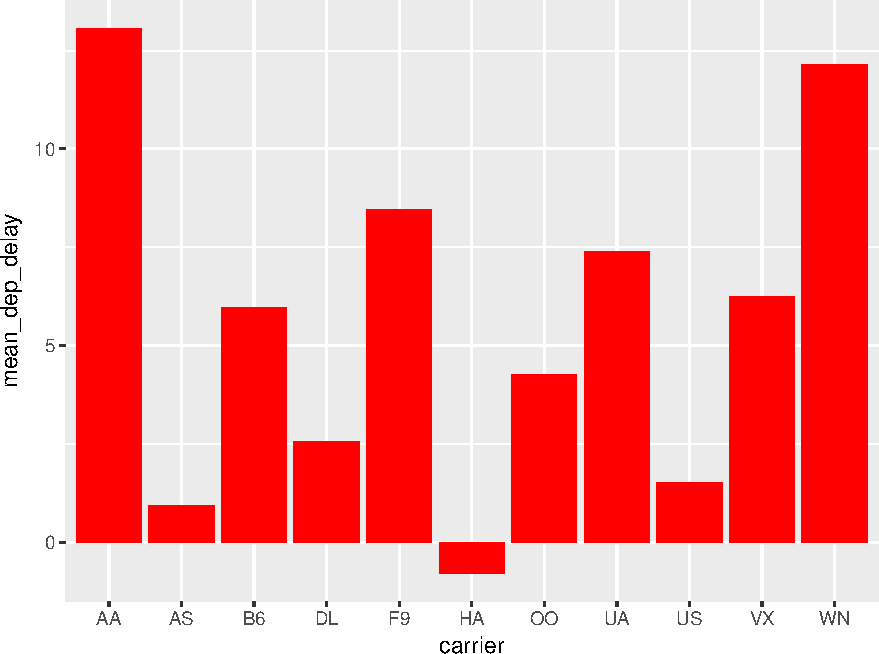
\includegraphics{thesis_files/figure-latex/delaysboxplot-1.pdf}
  \caption{\label{fig:delaysboxplot}Mean Delays by Airline}
  \end{figure}
  
  Here is a reference to this image: Figure \ref{fig:delaysboxplot}.
  
  A table linking these carrier codes to airline names is available at
  \url{https://github.com/ismayc/pnwflights14/blob/master/data/airlines.csv}.
  
  \clearpage
  
  Next, we will explore the use of the \texttt{out.extra} chunk option,
  which can be used to shrink or expand an image loaded from a file by
  specifying \texttt{"scale=\ "}. Here we use the mathematical graph
  stored in the ``subdivision.pdf'' file.
  
  \begin{figure}
  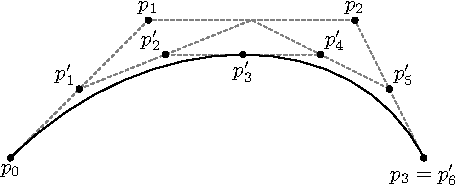
\includegraphics[scale=0.75]{figure/subdivision} \caption{Subdiv. graph}\label{fig:subd}
  \end{figure}
  
  Here is a reference to this image: Figure \ref{fig:subd}. Note that
  \texttt{echo=FALSE} is specified so that the \textbf{R} code is hidden
  in the document.
  
  \textbf{More Figure Stuff}
  
  Lastly, we will explore how to rotate and enlarge figures using the
  \texttt{out.extra} chunk option. (Currently this only works in the PDF
  version of the book.)
  
  \begin{figure}
  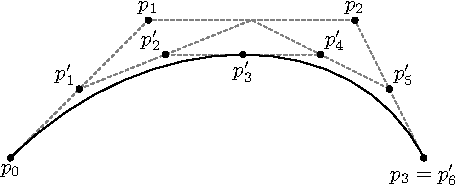
\includegraphics[angle=180, scale=1.1]{figure/subdivision} \caption{A Larger Figure, Flipped Upside Down}\label{fig:subd2}
  \end{figure}
  
  As another example, here is a reference: Figure \ref{fig:subd2}.
  
  \section{Footnotes and Endnotes}\label{footnotes-and-endnotes}
  
  You might want to footnote something.\footnote{footnote text} The
  footnote will be in a smaller font and placed appropriately. Endnotes
  work in much the same way. More information can be found about both on
  the CUS site or feel free to reach out to
  \href{mailto:data@reed.edu}{\nolinkurl{data@reed.edu}}.
  
  \section{Bibliographies}\label{bibliographies}
  
  Of course you will need to cite things, and you will probably accumulate
  an armful of sources. There are a variety of tools available for
  creating a bibliography database (stored with the .bib extension). In
  addition to BibTeX suggested below, you may want to consider using the
  free and easy-to-use tool called Zotero. The Reed librarians have
  created Zotero documentation at
  \url{http://libguides.reed.edu/citation/zotero}. In addition, a tutorial
  is available from Middlebury College at
  \url{http://sites.middlebury.edu/zoteromiddlebury/}.
  
  \emph{R Markdown} uses \emph{pandoc} (\url{http://pandoc.org/}) to build
  its bibliographies. One nice caveat of this is that you won't have to do
  a second compile to load in references as standard LaTeX requires. To
  cite references in your thesis (after creating your bibliography
  database), place the reference name inside square brackets and precede
  it by the ``at'' symbol. For example, here's a reference to a book about
  worrying: (Molina \& Borkovec, 1994). This \texttt{Molina1994} entry
  appears in a file called \texttt{thesis.bib} in the \texttt{bib} folder.
  This bibliography database file was created by a program called BibTeX.
  You can call this file something else if you like (look at the YAML
  header in the main .Rmd file) and, by default, is to placed in the
  \texttt{bib} folder.
  
  For more information about BibTeX and bibliographies, see our CUS site
  (\url{http://web.reed.edu/cis/help/latex/index.html})\footnote{Reed~College
    (2007)}. There are three pages on this topic: \emph{bibtex} (which
  talks about using BibTeX, at
  \url{http://web.reed.edu/cis/help/latex/bibtex.html}),
  \emph{bibtexstyles} (about how to find and use the bibliography style
  that best suits your needs, at
  \url{http://web.reed.edu/cis/help/latex/bibtexstyles.html}) and
  \emph{bibman} (which covers how to make and maintain a bibliography by
  hand, without BibTeX, at
  \url{http://web.reed.edu/cis/help/latex/bibman.html}). The last page
  will not be useful unless you have only a few sources.
  
  If you look at the YAML header at the top of the main .Rmd file you can
  see that we can specify the style of the bibliography by referencing the
  appropriate csl file. You can download a variety of different style
  files at \url{https://www.zotero.org/styles}. Make sure to download the
  file into the csl folder.
  
  \textbf{Tips for Bibliographies}
  
  \begin{itemize}
  \tightlist
  \item
    Like with thesis formatting, the sooner you start compiling your
    bibliography for something as large as thesis, the better. Typing in
    source after source is mind-numbing enough; do you really want to do
    it for hours on end in late April? Think of it as procrastination.
  \item
    The cite key (a citation's label) needs to be unique from the other
    entries.
  \item
    When you have more than one author or editor, you need to separate
    each author's name by the word ``and'' e.g.
    \texttt{Author\ =\ \{Noble,\ Sam\ and\ Youngberg,\ Jessica\},}.
  \item
    Bibliographies made using BibTeX (whether manually or using a manager)
    accept LaTeX markup, so you can italicize and add symbols as
    necessary.
  \item
    To force capitalization in an article title or where all lowercase is
    generally used, bracket the capital letter in curly braces.
  \item
    You can add a Reed Thesis citation\footnote{Noble (2002)} option. The
    best way to do this is to use the phdthesis type of citation, and use
    the optional ``type'' field to enter ``Reed thesis'' or
    ``Undergraduate thesis.''
  \end{itemize}
  
  \section{Anything else?}\label{anything-else}
  
  If you'd like to see examples of other things in this template, please
  contact the Data @ Reed team (email
  \href{mailto:data@reed.edu}{\nolinkurl{data@reed.edu}}) with your
  suggestions. We love to see people using \emph{R Markdown} for their
  theses, and are happy to help.
  
  \chapter*{Conclusion}\label{conclusion}
  \addcontentsline{toc}{chapter}{Conclusion}
  
  If we don't want Conclusion to have a chapter number next to it, we can
  add the \texttt{\{-\}} attribute.
  
  \textbf{More info}
  
  And here's some other random info: the first paragraph after a chapter
  title or section head \emph{shouldn't be} indented, because indents are
  to tell the reader that you're starting a new paragraph. Since that's
  obvious after a chapter or section title, proper typesetting doesn't add
  an indent there.
  
  \appendix
  
  \chapter{The First Appendix}\label{the-first-appendix}
  
  This first appendix includes all of the R chunks of code that were
  hidden throughout the document (using the \texttt{include\ =\ FALSE}
  chunk tag) to help with readibility and/or setup.
  
  \textbf{In the main Rmd file}
  
  \begin{Shaded}
  \begin{Highlighting}[]
  \CommentTok{# This chunk ensures that the thesisdown package is}
  \CommentTok{# installed and loaded. This thesisdown package includes}
  \CommentTok{# the template files for the thesis.}
  \NormalTok{if(!}\KeywordTok{require}\NormalTok{(devtools))}
    \KeywordTok{install.packages}\NormalTok{(}\StringTok{"devtools"}\NormalTok{, }\DataTypeTok{repos =} \StringTok{"http://cran.rstudio.com"}\NormalTok{)}
  \NormalTok{if(!}\KeywordTok{require}\NormalTok{(thesisdown))}
    \NormalTok{devtools::}\KeywordTok{install_github}\NormalTok{(}\StringTok{"ismayc/thesisdown"}\NormalTok{)}
  \KeywordTok{library}\NormalTok{(thesisdown)}
  \end{Highlighting}
  \end{Shaded}
  
  \textbf{In Chapter \ref{ref-labels}:}
  
  \begin{Shaded}
  \begin{Highlighting}[]
  \CommentTok{# This chunk ensures that the thesisdown package is}
  \CommentTok{# installed and loaded. This thesisdown package includes}
  \CommentTok{# the template files for the thesis and also two functions}
  \CommentTok{# used for labeling and referencing}
  \NormalTok{opts_chunk$}\KeywordTok{set}\NormalTok{(}\DataTypeTok{cache=}\OtherTok{TRUE}\NormalTok{)}
  
  \NormalTok{if(!}\KeywordTok{require}\NormalTok{(devtools))}
    \KeywordTok{install.packages}\NormalTok{(}\StringTok{"devtools"}\NormalTok{, }\DataTypeTok{repos =} \StringTok{"http://cran.rstudio.com"}\NormalTok{)}
  \NormalTok{if(!}\KeywordTok{require}\NormalTok{(dplyr))}
    \KeywordTok{install.packages}\NormalTok{(}\StringTok{"dplyr"}\NormalTok{, }\DataTypeTok{repos =} \StringTok{"http://cran.rstudio.com"}\NormalTok{)}
  \NormalTok{if(!}\KeywordTok{require}\NormalTok{(ggplot2))}
    \KeywordTok{install.packages}\NormalTok{(}\StringTok{"ggplot2"}\NormalTok{, }\DataTypeTok{repos =} \StringTok{"http://cran.rstudio.com"}\NormalTok{)}
  \NormalTok{if(!}\KeywordTok{require}\NormalTok{(ggplot2))}
    \KeywordTok{install.packages}\NormalTok{(}\StringTok{"bookdown"}\NormalTok{, }\DataTypeTok{repos =} \StringTok{"http://cran.rstudio.com"}\NormalTok{)}
  \NormalTok{if(!}\KeywordTok{require}\NormalTok{(thesisdown))\{}
    \KeywordTok{library}\NormalTok{(devtools)}
    \NormalTok{devtools::}\KeywordTok{install_github}\NormalTok{(}\StringTok{"ismayc/thesisdown"}\NormalTok{)}
  \NormalTok{\}}
  \KeywordTok{library}\NormalTok{(thesisdown)}
  \KeywordTok{library}\NormalTok{(pcadapt)}
  \KeywordTok{library}\NormalTok{(EILA)}
  \KeywordTok{library}\NormalTok{(simulate)}
  \NormalTok{flights <-}\StringTok{ }\KeywordTok{read.csv}\NormalTok{(}\StringTok{"data/flights.csv"}\NormalTok{)}
  \end{Highlighting}
  \end{Shaded}
  
  \chapter{The Second Appendix, for
  Fun}\label{the-second-appendix-for-fun}
  
  \backmatter
  
  \chapter*{References}\label{references}
  \addcontentsline{toc}{chapter}{References}
  
  \noindent
  
  \setlength{\parindent}{-0.20in} \setlength{\leftskip}{0.20in}
  \setlength{\parskip}{8pt}
  
  \hypertarget{refs}{}
  \hypertarget{ref-alexander2009}{}
  Alexander, D. (2009). \emph{Fast model-based estimation of ancestry in
  unrelated individuals.}
  
  \hypertarget{ref-angel2000}{}
  Angel, E. (2000). \emph{Interactive computer graphics : A top-down
  approach with opengl}. Boston, MA: Addison Wesley Longman.
  
  \hypertarget{ref-angel2001}{}
  Angel, E. (2001a). \emph{Batch-file computer graphics : A bottom-up
  approach with quicktime}. Boston, MA: Wesley Addison Longman.
  
  \hypertarget{ref-angel2002a}{}
  Angel, E. (2001b). \emph{Test second book by angel}. Boston, MA: Wesley
  Addison Longman.
  
  \hypertarget{ref-caye2016}{}
  Caye, K. (2016). \emph{TESS3: Fast inference of spatial population
  structure and genome scans for selection.}
  
  \hypertarget{ref-frichot2015}{}
  Frichot, É. (2015). \emph{LEA: An r package for landscape and ecological
  association studies.}
  
  \hypertarget{ref-maples2013}{}
  Maples, B. K. (2013). \emph{RFMix: A discriminative modeling approach
  for rapid and robust local-ancestry inference.}
  
  \hypertarget{ref-mcvean2009}{}
  McVean, G. (2009). A genealogical interpretation of principal components
  analysis.
  
  \hypertarget{ref-Molina1994}{}
  Molina, S. T., \& Borkovec, T. D. (1994). The Penn State worry
  questionnaire: Psychometric properties and associated characteristics.
  In G. C. L. Davey \& F. Tallis (Eds.), \emph{Worrying: Perspectives on
  theory, assessment and treatment} (pp. 265--283). New York: Wiley.
  
  \hypertarget{ref-noble2002}{}
  Noble, S. G. (2002). \emph{Turning images into simple line-art}
  (Undergraduate thesis). Reed College.
  
  \hypertarget{ref-price2009}{}
  Price, A. L. (2009). \emph{Sensitive detection of chromosomal segments
  of distinct ancestry in admixed populations.}
  
  \hypertarget{ref-reedweb2007}{}
  Reed~College. (2007, march). LaTeX your document. Retrieved from
  \url{http://web.reed.edu/cis/help/LaTeX/index.html}
  
  \hypertarget{ref-suarez2016}{}
  Suarez-Gonzalez, et a., Adriana. (2016). Genomic and functional
  approaches reveal a case of adaptive introgression from populus
  balsamifera (balsam poplar) in p. trichocarpa (black cottonwood).
  \emph{Molecular Ecology}, 2427--2442.
  
  \hypertarget{ref-thornton2014}{}
  Thornton, T. (2014). \emph{Local and global ancestry inference, and
  applications to genetic association analysis for admixed populations.}
  
  \hypertarget{ref-yang2013}{}
  Yang, J. J. (2013). \emph{Efficient inference of local ancestry.}


  % Index?

\end{document}

